\section{Einführung in die Bionik - Biologie im Überblick}

\textbf{Was ist Bionik?} Bionik (im Englischen: Biomimetics/ biomimesis/ biomimikry/ bio-inspired) ist die Komposition aus Biologie und Technik. Lebewesen dienen als Ideengeber für technische Umsetzungen, sind aber nicht in die Herstellung bionischer Produkte eingebunden. Keine direkte Übertragung, sondern ein kreatives Umsetzen in die Technik, d.h. ein durch die Natur angeregtes „Neuerfinden“.

Im Gegensatz dazu steht die \textbf{Biotechnologie}: Nutzung von Lebewesen oder von lebenden Subsystemen von Lebewesen für die Produktion der gewünschten Stoffe oder den Abbau unerwünschter Substanzen.
\\
\\
Als \textbf{Mimese} wird eine Form der Tarnung bezeichnet, bei der ein Lebewesen in Gestalt, Farbe und Haltung einen Teil seines Lebensraumes annimmt.

\begin{center}
	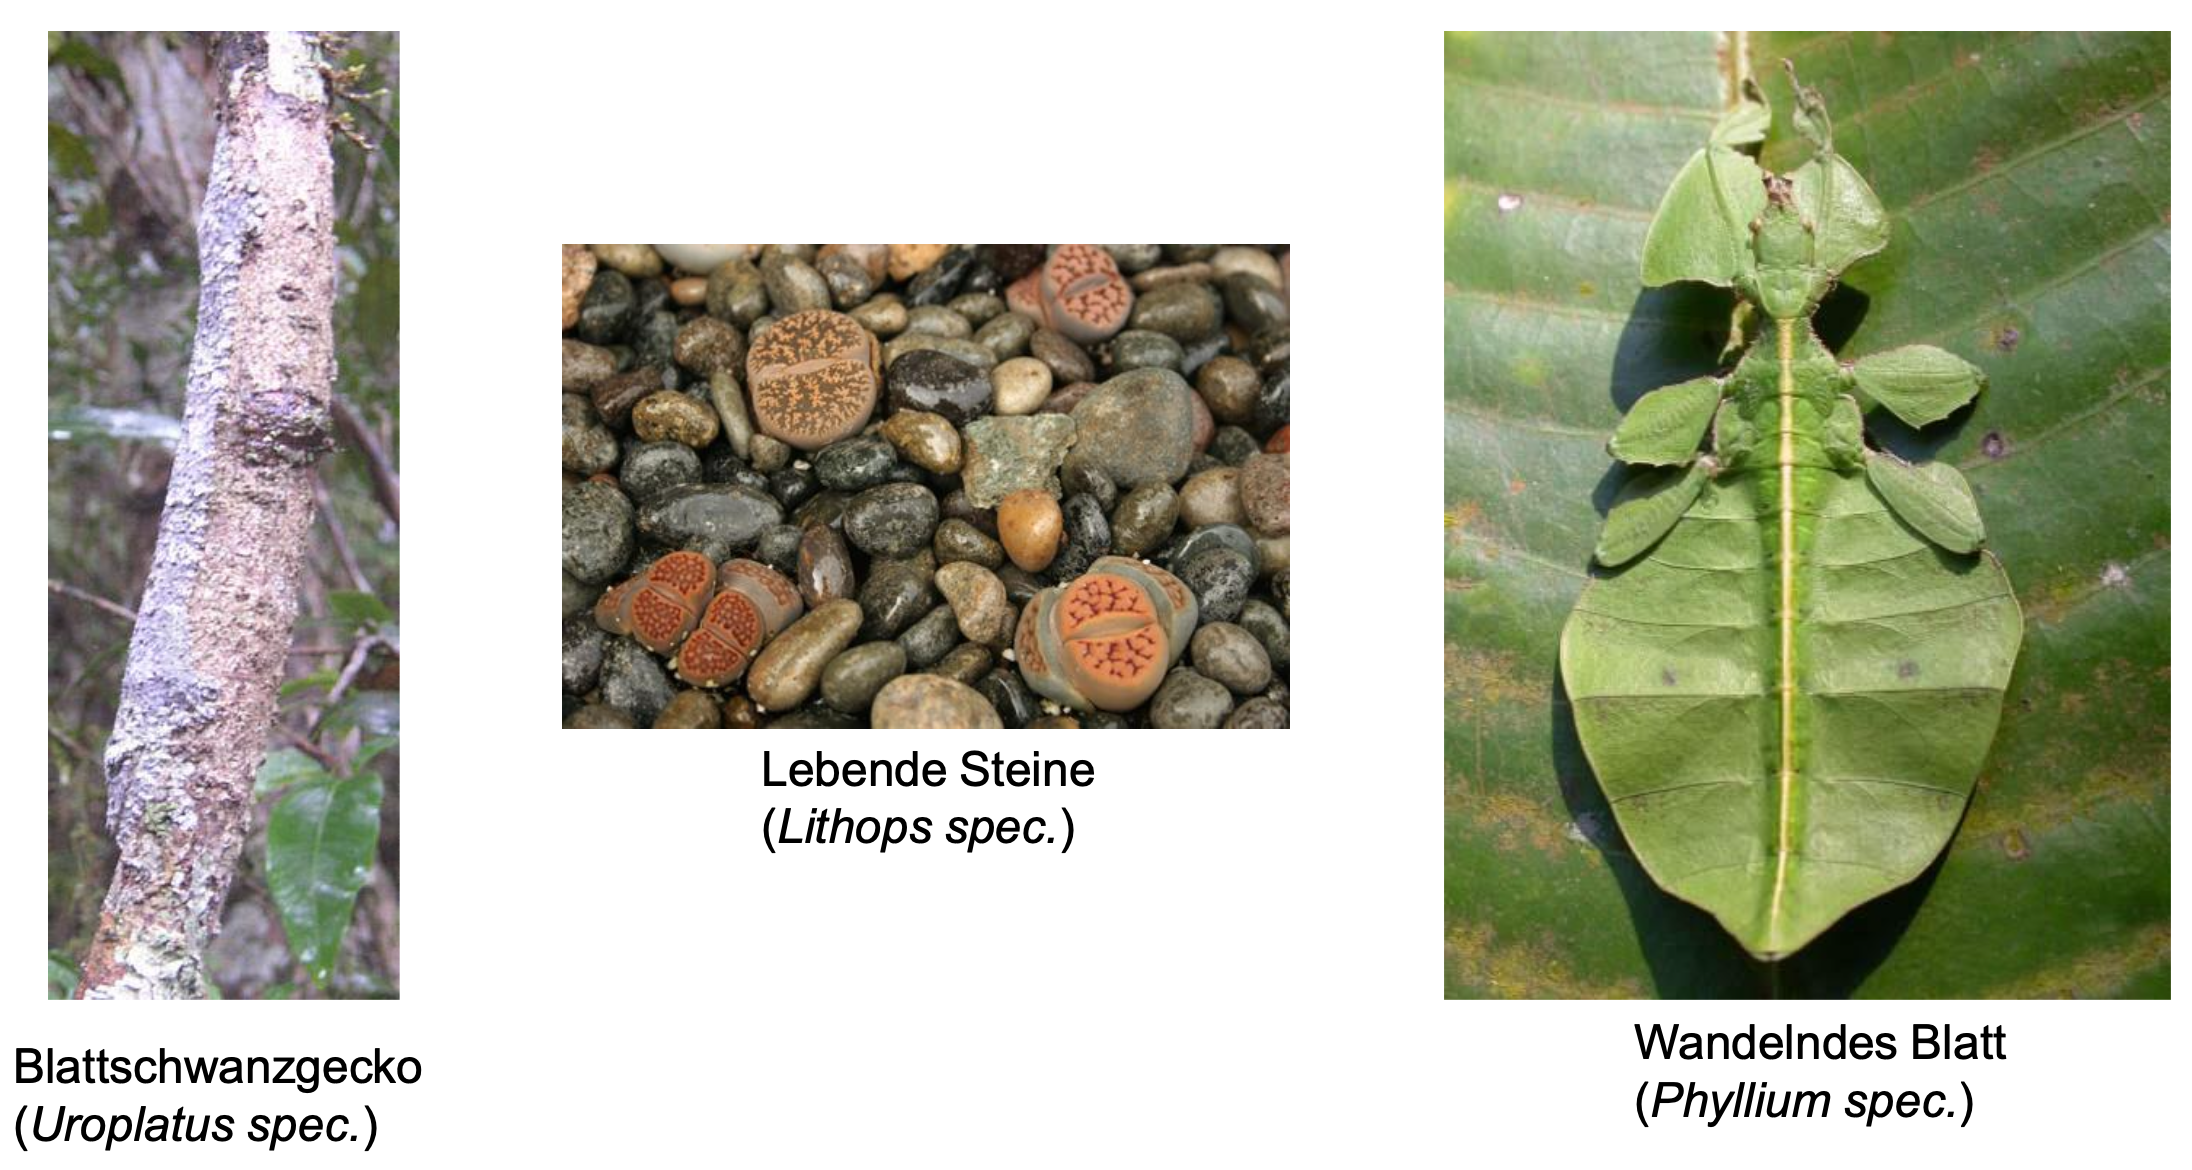
\includegraphics[width=8cm]{lec1/figures/Mimese.png}	
\end{center}
\textbf{Bates'sche Mimikry}: Ähnlichkeit von zwei Tierarten, wobei ein Tier ein ungenießbares Tier nachahmt.\\
\textbf{Mertens'sche Mimikry}: Ähnlichkeit von zwei Tierarten, wobei ein Tier ein giftiges Tier nachahmt. Dabei ahmen Tierarten vor allem mäßig giftige Tiere nach, da Angreifer nur bei diesen aus nicht-tödlichen Interaktionen lernen können.\\
\textbf{Peckham'sche Mimikry}: „Aggressive Mimikry“ die potentielle Beutetiere anlockt (z.B.\ Angel beim Seeteufel).

\subsection{Teilbereiche der Bionik}
Es werden folgende Beispiele genannt:
\begin{enumerate}
	\item \textbf{Leichtbau \& Materialien}: Selbstschärfende Messer für Industrieschneidemaschinen am Vorbild von Zähnen von Nagetieren. Dabei wird für die Spanfläche ein weiches Material und für die Freifläche ein hartes Material gewählt, sodass bei Abnutzung der Spanfläche die scharfe Schnittkante erhalten bleibt.
	\item \textbf{Oberflächen}: Selbstreinigende Oberflächen am Vorbild vom Lotus-Effekt and Blattoberflächen.
	\item \textbf{Fluiddynamik, Schwimmen \& Fliegen}: Der Kofferfisch hat einen geringen Strömungswiderstand (trotz seinen recht großen Körper). Diese Eigenschaft kann z.B. im Karosseriebau verwendet werden.
	\item \textbf{Biomechatronik \& Robotik}: Sechs- und mehrbeinige Tiere sind auch im Stand stabil (\textit{statisch stabile Gangart}). Vier- und zweibeinige Tiere sind dagegen nur bei Bewegung stabil (\textit{dynamisch stabile Gangart}).
	\item \textbf{Kommunikation \& Sensorik}: Das Infrarot-Organ des Schwarzen Kiefernprachkäfers kann als Vorbild für einen IR-Sensor verwendet werden.
	\item \textbf{Optimierung}: Die Struktur von Bäumen und Knochen kann zur Form- und Gewichtsoptimierung im Leichtbau verwendet werden ($\rightarrow$ Methode der Zugdreiecke nach dem Vorbild der gerundeten Ausformung von Astgabelungen).
	\item \textbf{Architektur \& Design}: Optimierung von Gebäudestrukturen (Leichtbau/ Ressourcenschonung/ hohe Stabilität).
\end{enumerate}

\subsection{Das Forschungsprinzip Bionik}

Biologen/ Grundlagenforscher verfolgen das bottom-up Prinzip:
\begin{center}
	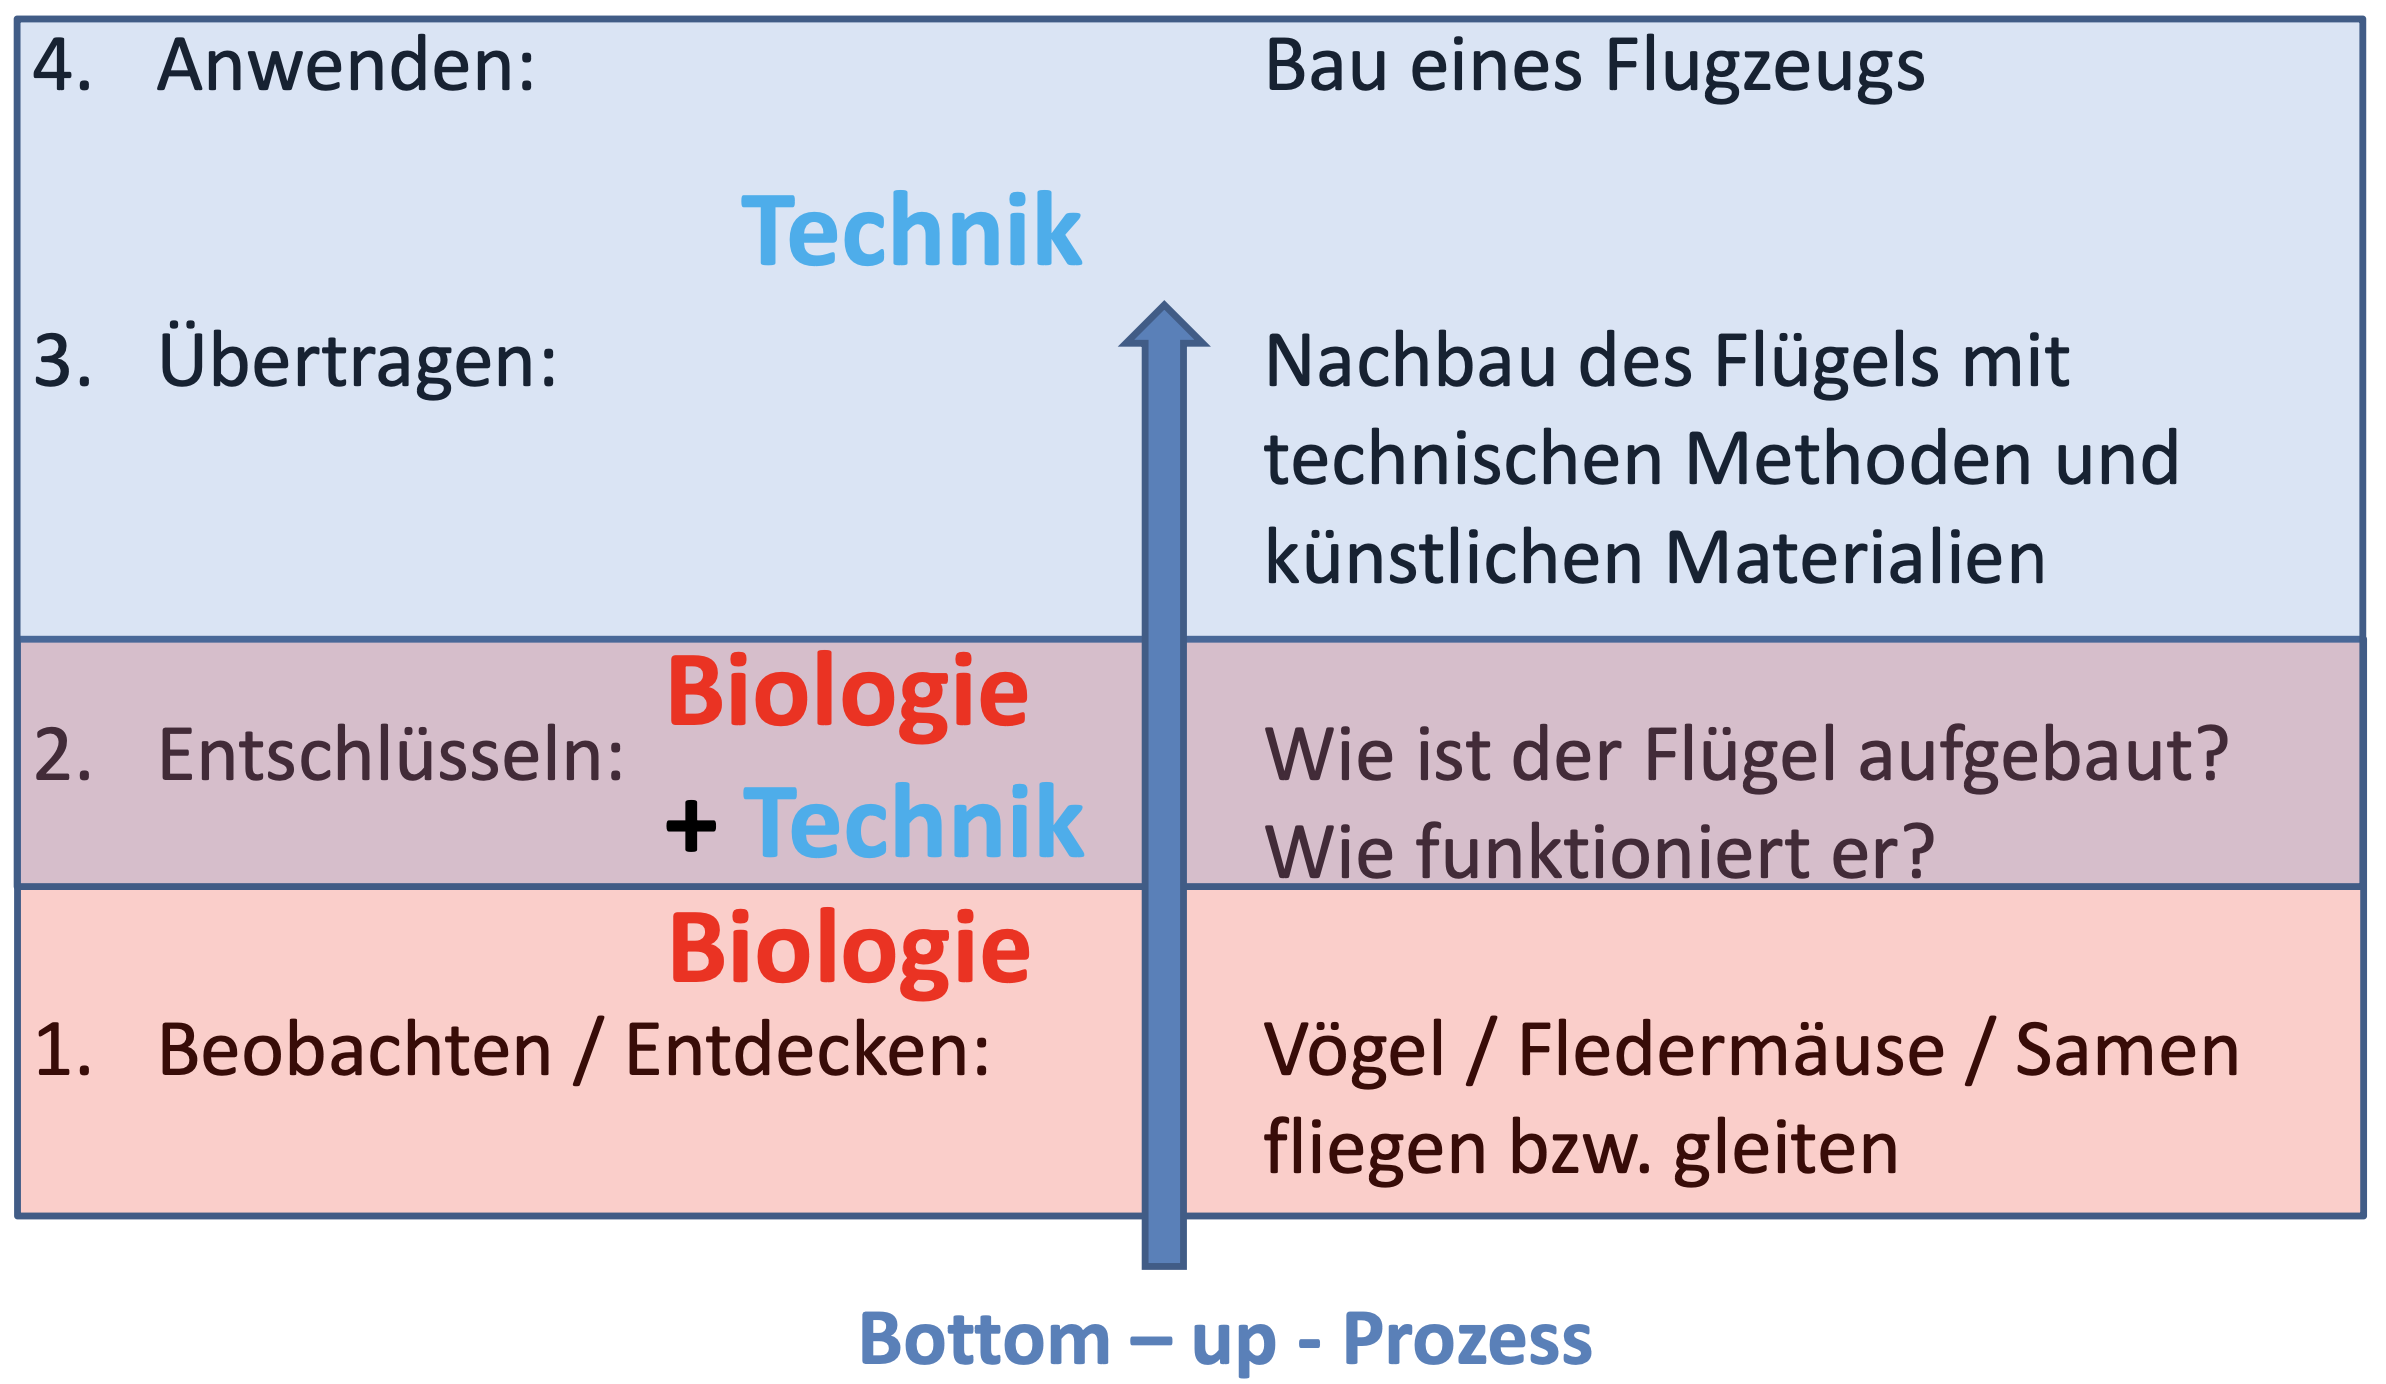
\includegraphics[width=10cm]{lec1/figures/Forschungsprinzip.png}	
\end{center}
Vorteile: Große Innovationshöhe. Nachteile: Erfolg/ Zeitbedarf sind nicht abschätzbar. ROI ist nicht gesichert.\\
Der Ingenieur wird vom Optimierungsproblem her top-down getrieben:

\begin{center}
	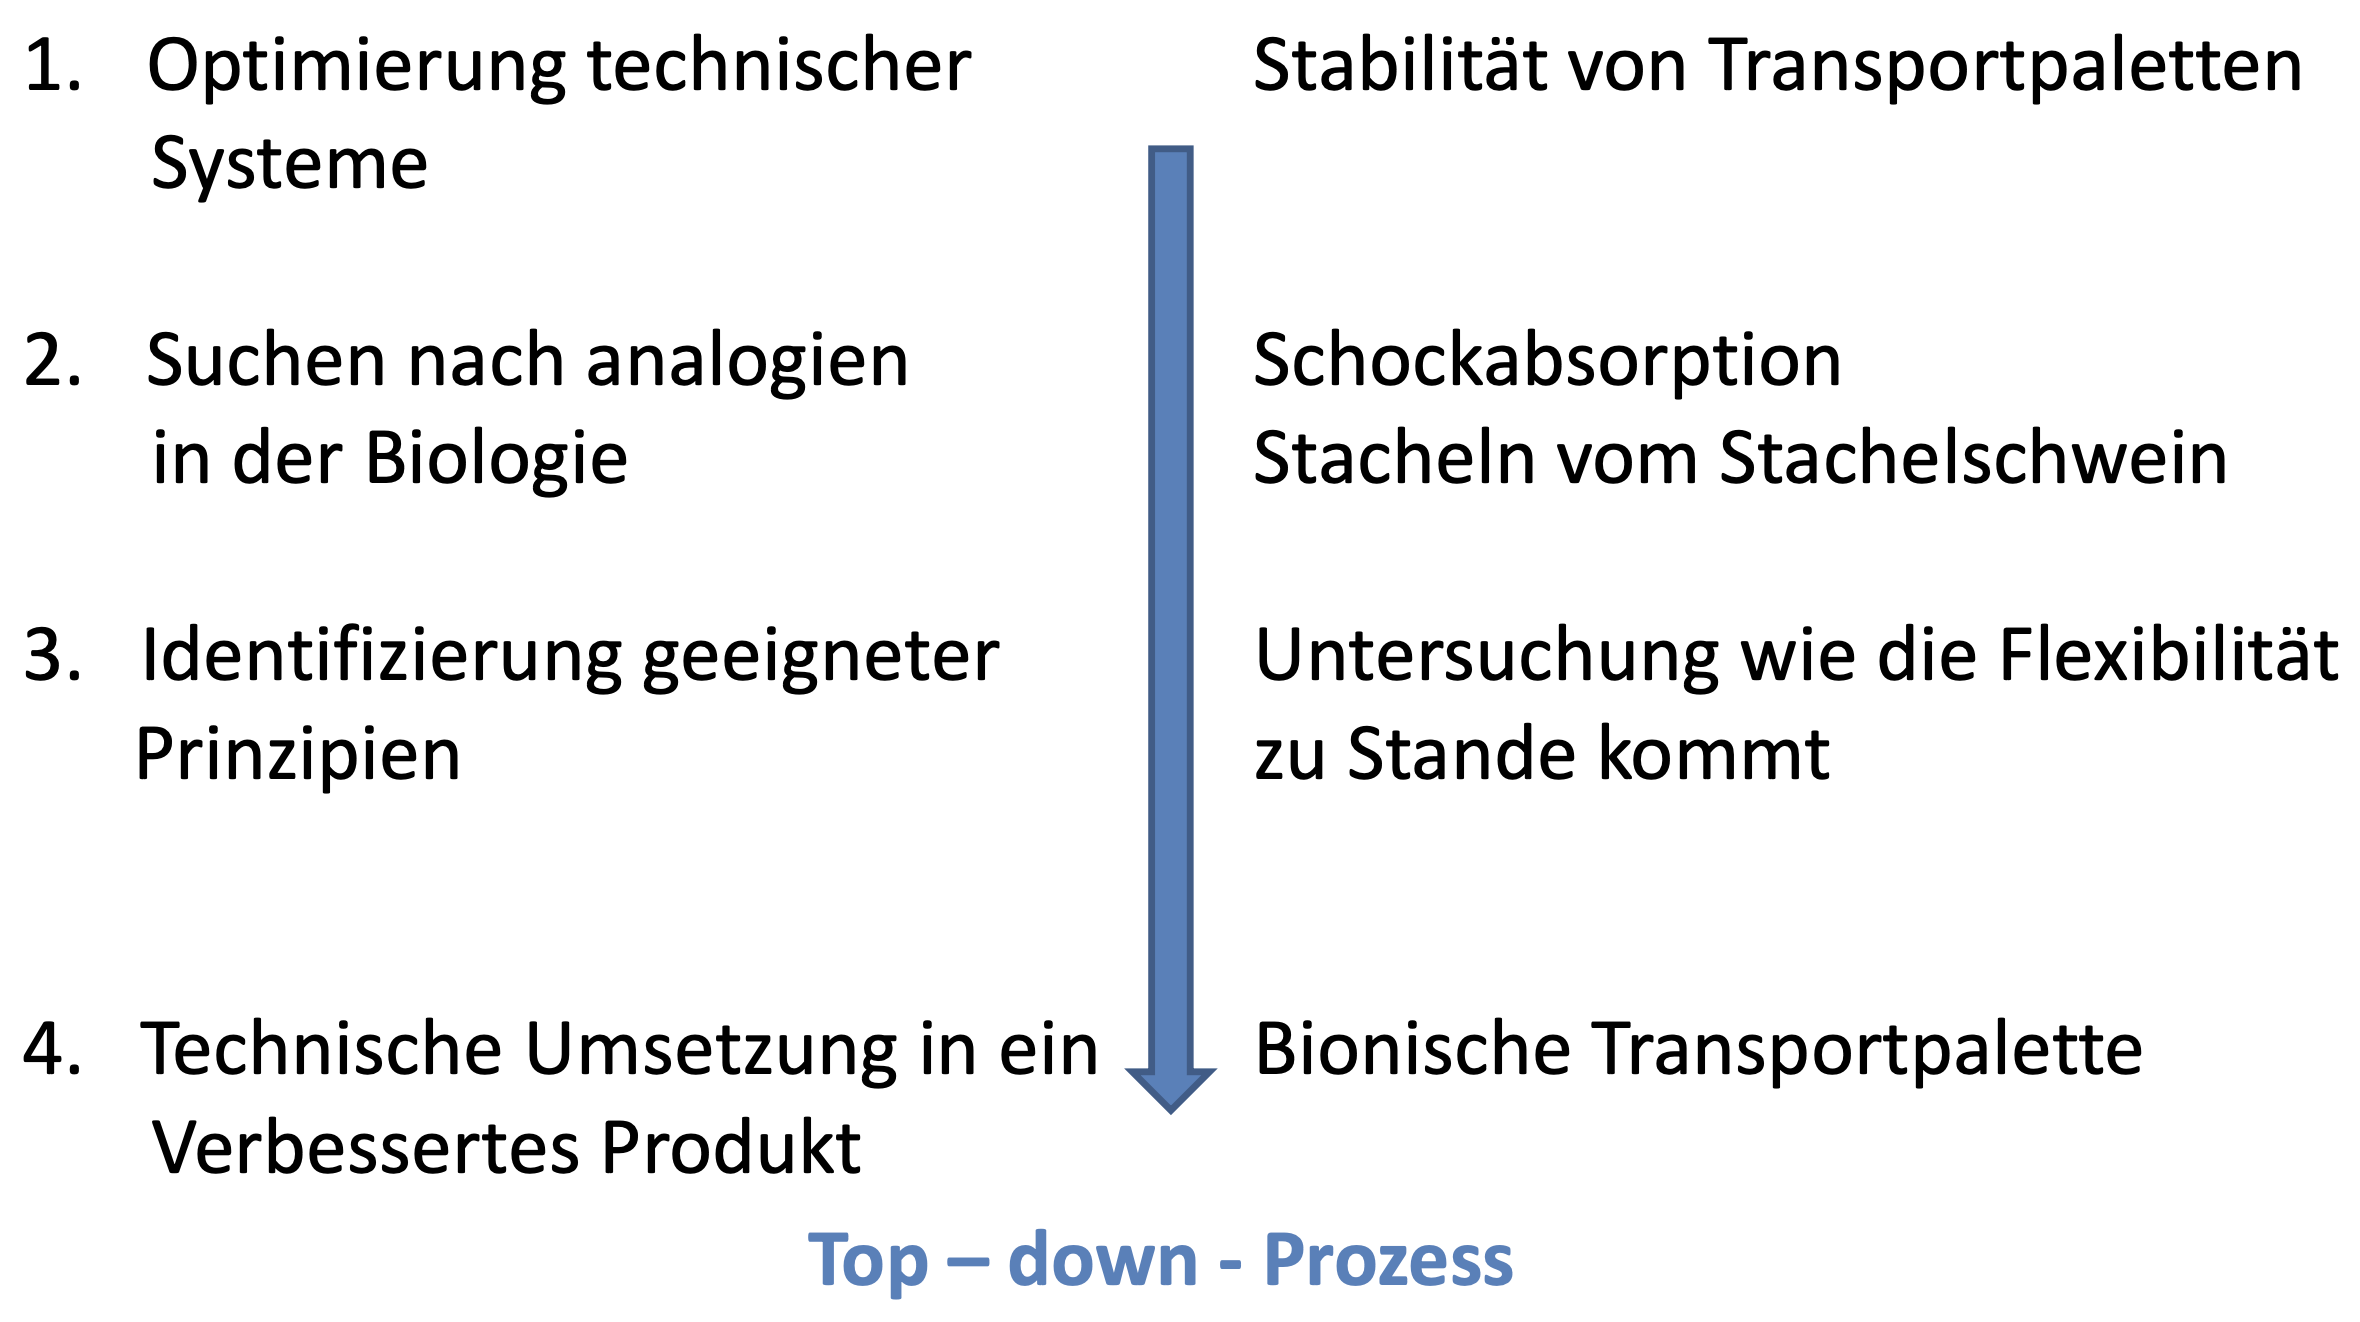
\includegraphics[width=10cm]{lec1/figures/top-down.png}
\end{center}
Vorteile: Erfolg/ Zeitbedarf sind abschätzbar. ROI ist gesichert. Nachteile: Geringe Innovationshöhe.
\\
\\
Die Technische Biologie, Bionik und Reverse Bionik sind durch eine geschlossene Spirale verbunden:
\begin{center}
	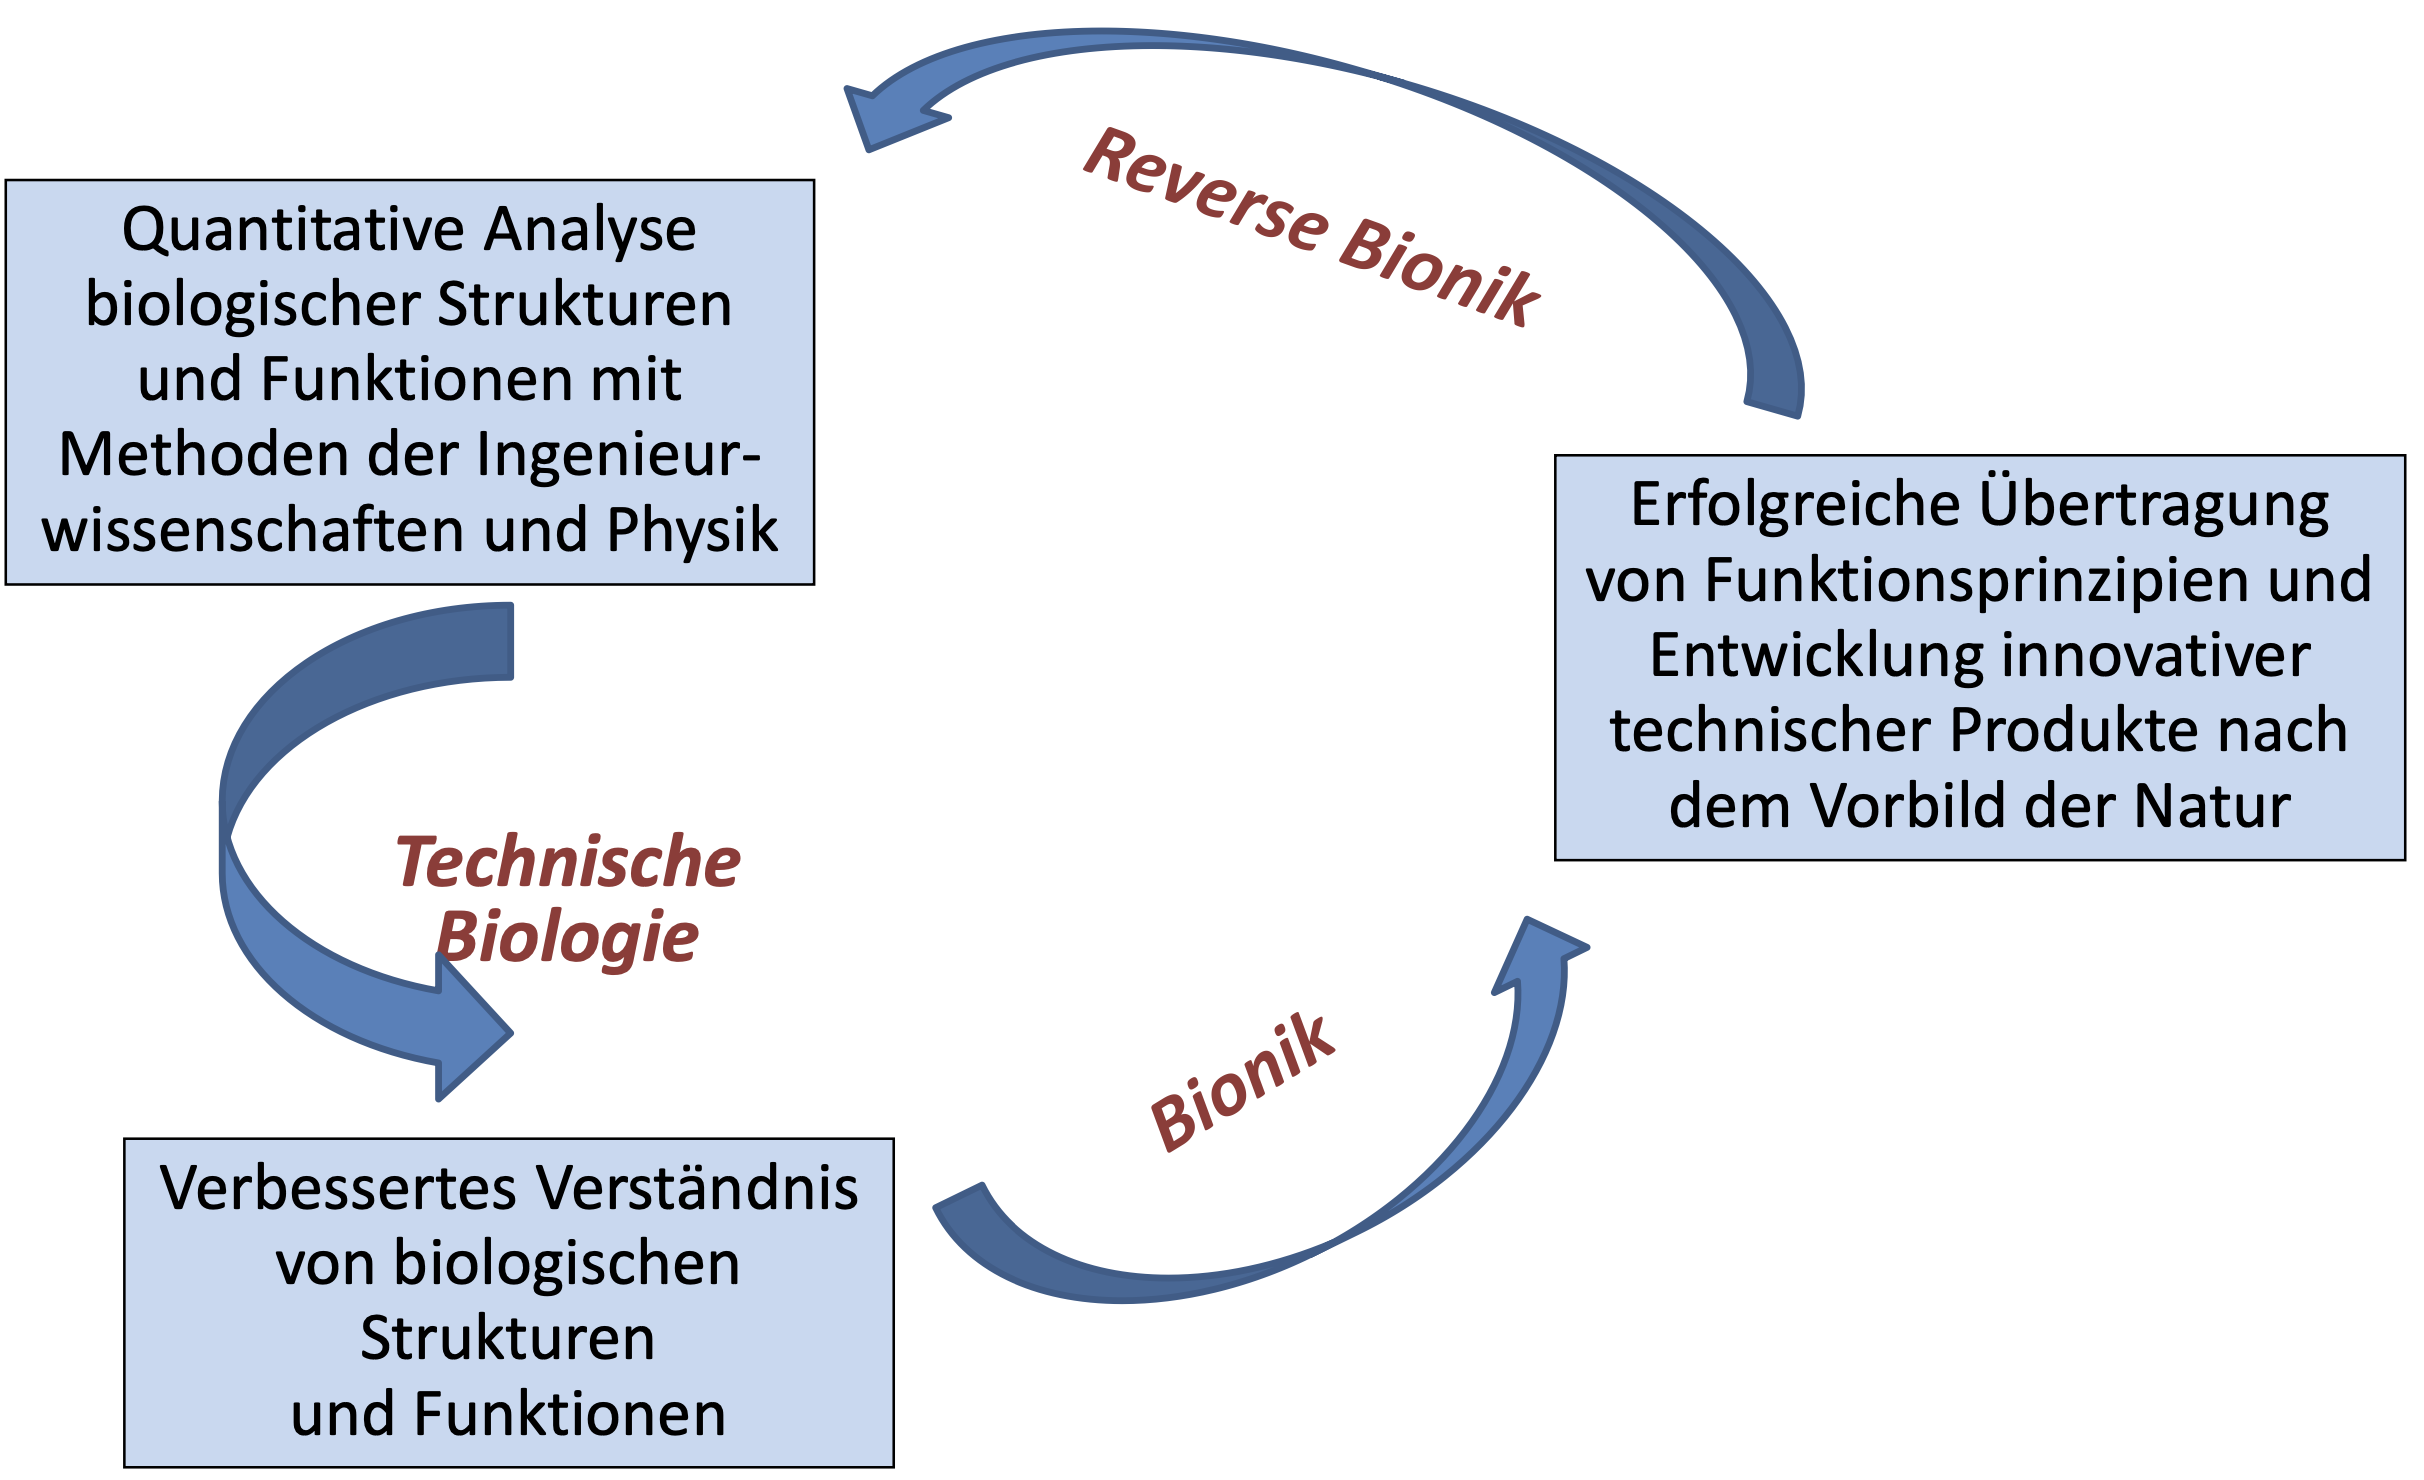
\includegraphics[width=10cm]{lec1/figures/spirale.png}
\end{center}

\subsection{Biologische Grundlagen}
Während bei der technischen Produktherstellung (Sägen, Stanzen, Schneiden, etc.) das Endprodukt aus einem Werkstückrohling i.d.R.\ durch Abtragung von Material geschieht, entstehen biologische Produkte durch \textit{genetische kontrollierte Selbstorganisation} (Molekül $\rightarrow$ Organell $\rightarrow$ Zelle $\rightarrow$ Gewebe $\rightarrow$ Organ $\rightarrow$ Spezies). 3D-Drucker imitieren hier eher die biologische Produktherstellung.
\\
\\
Was ist eine \textbf{Spezies}? Nach dem \textbf{Morphologischen Artkonzept} geschieht die Unterscheidung anhand von morphologischen (äußeren) Merkmalen. Das \textbf{Ethologischen Artkonzept} trifft die Unterscheidung anhand des Verhaltens. Beim \textbf{Populationsgentischen Artkonzept} ist das entscheidende Merkmal, ob sich Populationen zweier Arten miteinander fortpflanzen können (``Biospezies''). Geographische/ ökologische Isolation zweier Populationen kann langfristig auch zur reproduktiven Isolation führen. 

Nachkommen zweier Spezies werden \textit{Allospezies} genannt, wenn sie fertil sind, und \textit{Hybride} wenn nicht. Es gibt allerdings auch Spezies, die sich nicht mit dem Populationsgenetischen Artkonzept abgrenzen lassen (z.B. Bakterien).
\\
\\
Der Census of marine life schätzt die \textbf{Artenvielfalt} auf ca.\ 8,7 Mio.\ Spezies, wovon lediglich 1,2 Mio. beschrieben sind (60\% davon Insekten). Die biologischen Hot-Spots sind der tropische Regenwald aber auch z.B. das Mittelmeer:

\begin{center}
	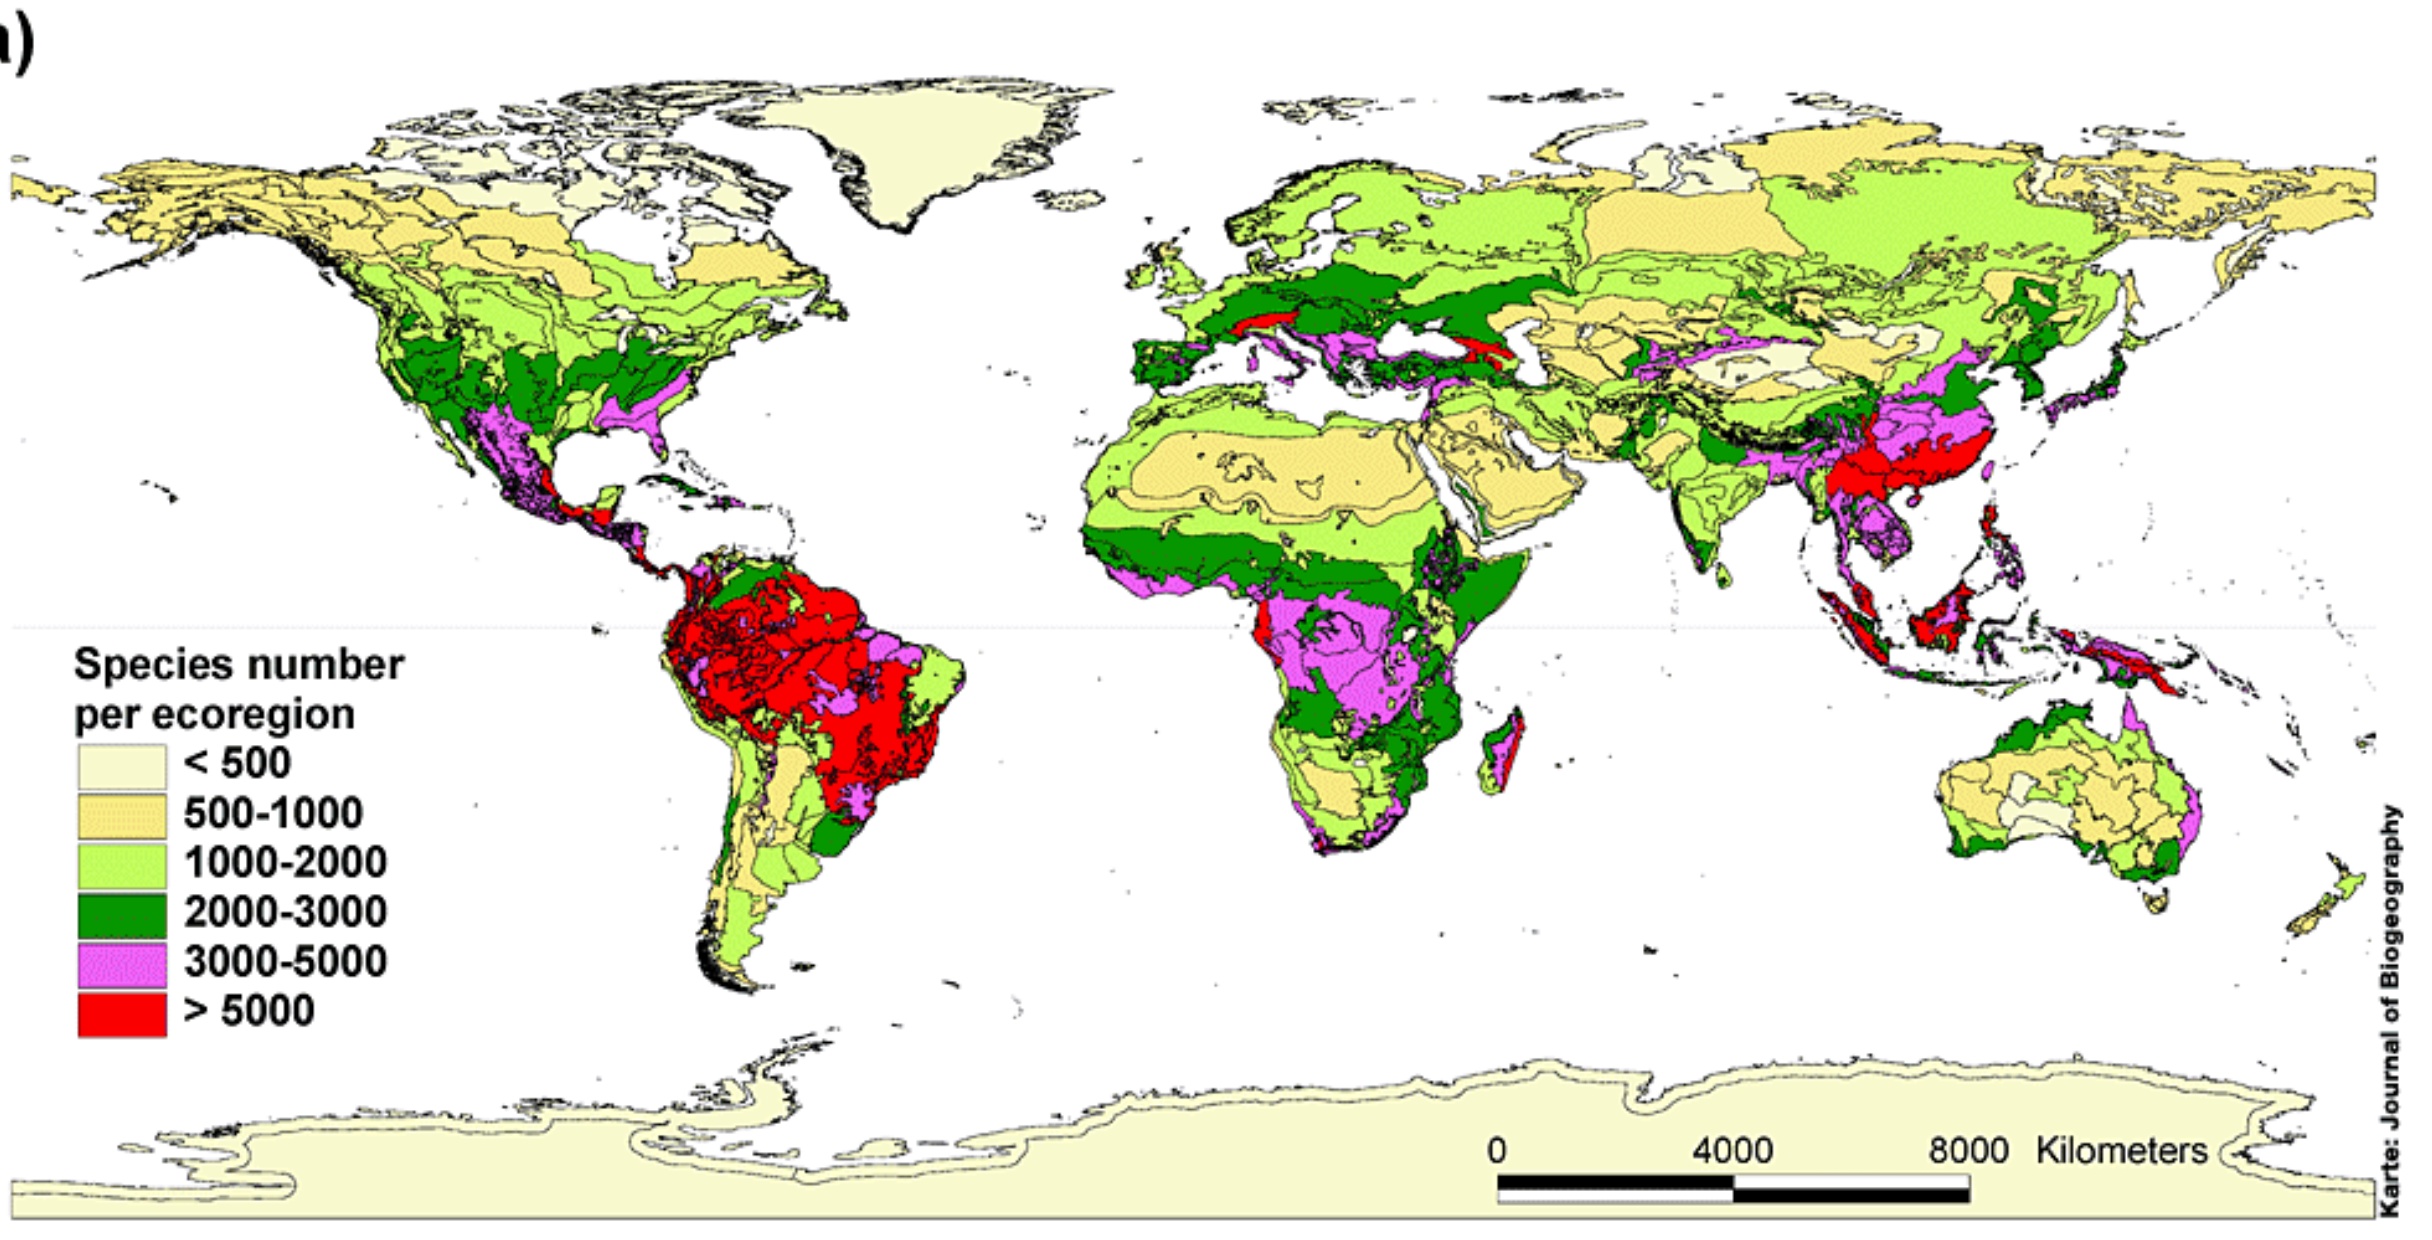
\includegraphics[width=10cm]{lec1/figures/bio-hotspots.png}
\end{center} 
Gerade diese Gebiete sind allerdings auch von Waldbränden besonders bedroht. 
\\
\\
\subsubsection{Systematik der Arten}

Klassischerweise erfolgt die Bestimmung und Benennung von Arten nach der Systematik: Gattungsname, Artenname, Unterart (weitere veraltete Einteilungen). Heute folgt man der \textbf{Phylogenetische Systematik}, wobei die Verwandschaftsbeziehung zwischen den Arten dargestellt wird. Dabei entstammen jeder Verzweigung immer zwei Äste und jeder Ast wird durch ein abgeleitetes Merkmal begründet.

\begin{center}
		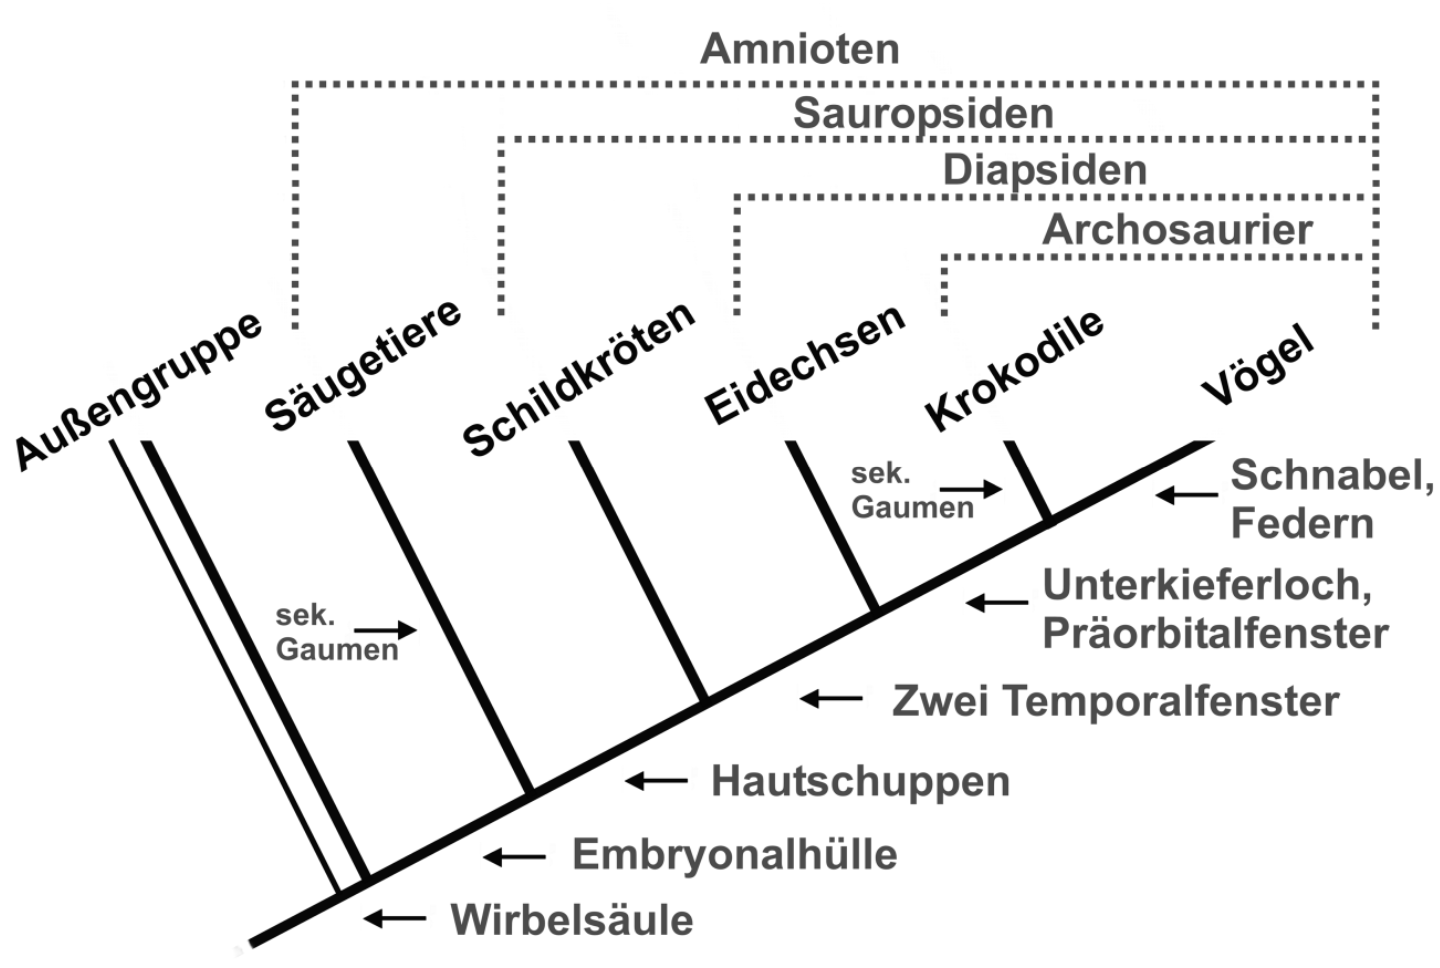
\includegraphics[width=9cm]{lec1/figures/phylogenetische_systematik.png}
\end{center}
\begin{center}
	\begin{itemize}
		\item \textbf{Apomorphie}: Merkmal welches im Vergleich zum direkten Vorfahren neu erworben wurde („abgeleitetes Merkmal“) $\rightarrow$ beim Vogel: Schnabel, Federn.
		\item \textbf{Plesiomorphie}: Gegenbegriff zur Apomorphie. Merkmal, welches bereits vor der Abstammungslinie entstanden ist („ursprüngliches Merkmal“) $\rightarrow$ beim Vogel: z.B. Wirbelsäule.
		\item \textbf{Schhwestergruppen}: Aufspaltung einer Stammart in zwei Gruppen aus einem gemeinsamen unmittelbaren Vorfahren. $\rightarrow$ z.B. Krokodile und Vögel
		\item \textbf{Synapomorphie}: Gemeinsamer Besitz eines apomorphen Merkmals $\rightarrow$ z.B. Unterkieferloch, Präorbitalfenster bei Krokodilen und Vögeln
		\item \textbf{Monophyletische Gruppe}: Systematische Einheit, die den gemeinsamen Vorfahren und alle seine Nachfahren enthält. $\rightarrow$ z.B. Krokodile, Vögel
		\item \textbf{Paraphyletische Gruppe}: Systematische Gruppe, die den gemeinsamen Vorfahren aber nicht alle Nachfahren enthält. $\rightarrow$ z.B. Schildkröten, Eidechsen und Krokodile (Vögel fehlen)
		\item \textbf{Analogie}: Durch \textit{konvergente Entwicklung} entstandene Merkmale, die unabhängig voneinander entstanden sind. Erfüllen die gleiche Aufgabe sind aber nicht auf einen gemeinsamen Vorfahren zurückzuführen. $\rightarrow$ sek. Gaumen bei Säugetieren und Krokodilen. (Diese Eigenschaften sind in der Bionik besonders interessant)
	\end{itemize}
\end{center}

\subsubsection{Entstehung von Merkmalen}

Die Organismen, welche am besten an ihre Umgebung angepasst sind, werden durch die natürliche Selektion begünstigt und vererben Eigenschaften an ihre Nachkommen. Bei der Vererbung kann neben der Weitergabe der Merkmale and Nachkommen, genetische Variabilität durch Mutationen der DNA entstehen.
Die Variabilität der Individuen führt zu unterschiedlichen
Überlebensraten und Fortpflanzungserfolg und damit zur \textbf{natürlichen Selektion}. Individuen mit Merkmalen, die zu einer bessere Anpassung an die Umwelt führen treten in der nächsten Generation vermehrt auf.
\\
\\
\textbf{Selektionsfaktoren} (Umweltfaktoren mit Einfluss auf die ``Fitness'' eines Individuums):
\begin{itemize}
	\item Abiotisch: Licht, Temperatur, Drucke, Feuchtigkeit, Wind
	\item Biotisch: Zwischenartlich und innerartlich
	\item Künstlich: Zucht durch Menschen
\end{itemize}
\textbf{Sexuelle Selektion}: Auslese von Individuen durch Vorteile beim Fortpflanzungserfolg gegenüber Geschlechtsgenossen derselben Art.

\subsection{Fehleinschätzungen \& Grenzen der Bionik}

3 Fehleinschätzungen:
\begin{enumerate}
	\item Bionik liefert optimale Lösungen. (``optimiert ist nicht optimal'')
	\item Bionik ist ressourcenschonen umweltfreundlich
	\item Bionik besteht vor allem aus Übertragung von Technik (ist vor allem Grundlagenforschung)
\end{enumerate}
Grenzen: Die Evolution hat keine Richtung und ist ein dynamischer Prozess. D.h.\ Merkmale werden nur soweit wie nötig optimiert und es können alternative Entwicklungsformen entstehen, wenn diese optimaler als Hochleistungsmerkmale sind. Wie z.B. bei der Kerguelen-Fliege, die in einer stark windigen Umgebung ihre Flügel zurückgebildet hat (und nun am Boden lebt), anstatt stärkere zu entwickeln. 
\begin{center}
	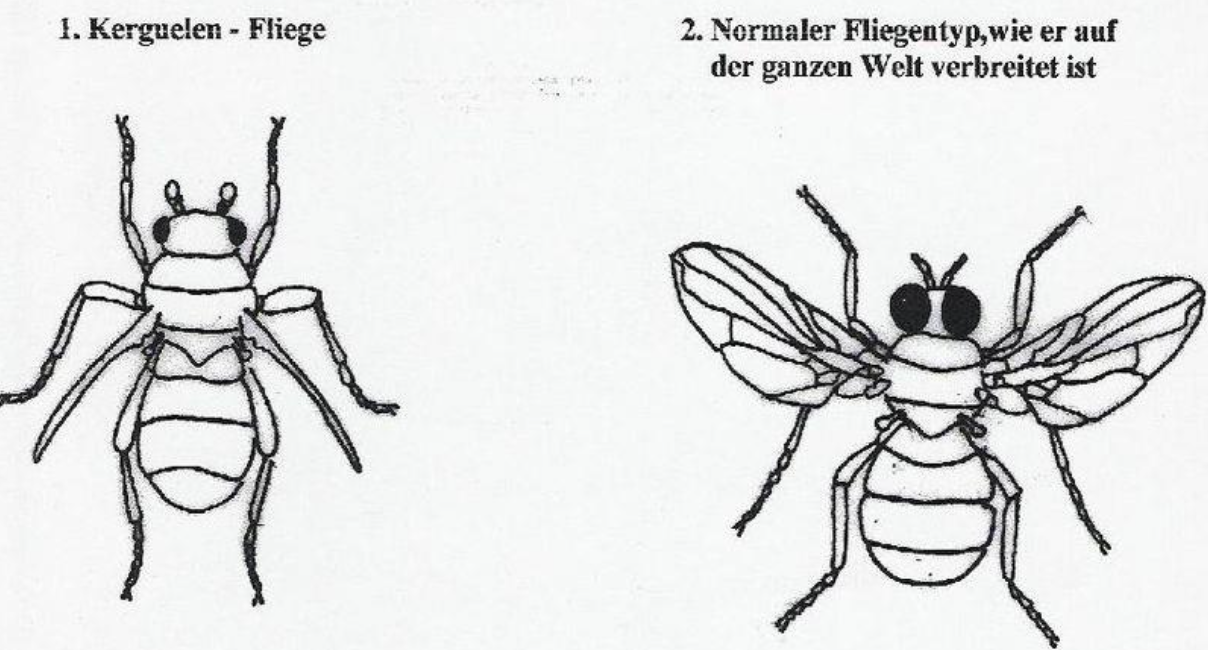
\includegraphics[width=6cm]{lec1/figures/fliege.png}
\end{center}
